\documentclass{beamer}
\usepackage[utf8]{inputenc}
\usepackage[czech]{babel}
\usepackage[IL2]{fontenc}
\usepackage{graphicx}
\usepackage[noend, ruled, linesnumbered]{algorithm2e}
\usepackage{amssymb}
\usepackage{changepage}

\graphicspath{ {./img/} }

\title{Grafové algoritmy -- Dijkstrův algoritmus}
\subtitle{ITY -- 5. projekt}
\author{Jakub Hlava}
\date{2020}
\institute[FIT VUT]{Vysoké učení technické \\ Fakulta informačních technologií}

\usetheme{Madrid}

\renewcommand{\algorithmcfname}{Algoritmus}

\begin{document}

\maketitle

\section{Dijkstrův algoritmus}
\subsection{Popis problému}
\frame {
    \frametitle{Co jsou to vlastně grafy?}
    \begin{itemize}
        \item Graf podle teorie grafů je dvojice, kterou tvoří:
        \begin{itemize}
            \item Množina hran
            \begin{itemize}
                \item Mohou být orientované (pak je i graf orientovaný) nebo neorientované
                \item Mohou a nemusí mít váhu
            \end{itemize}
            \item Množina vrcholů
        \end{itemize}
        \item Grafy se používají pro zápis, zobecnění a zjednodušení různých problémů
        \item Jako příklad můžeme do grafu rozebrat třeba ulice ve městě
        \begin{itemize}
            \item Vrcholy grafu budou křižovatky ulic
            \item Samotné ulice budou hranami grafu
            \item Pokud si do grafu přidáme i orientované hrany, pak nimi můžeme zaznačit třeba jednosměrnou ulici
            \item Váhami hran se pak stanou délky ulic od křižovatky ke křižovatce
        \end{itemize}
    \end{itemize}
}
\frame{
    \frametitle{Příklad grafu města}
    \centering
    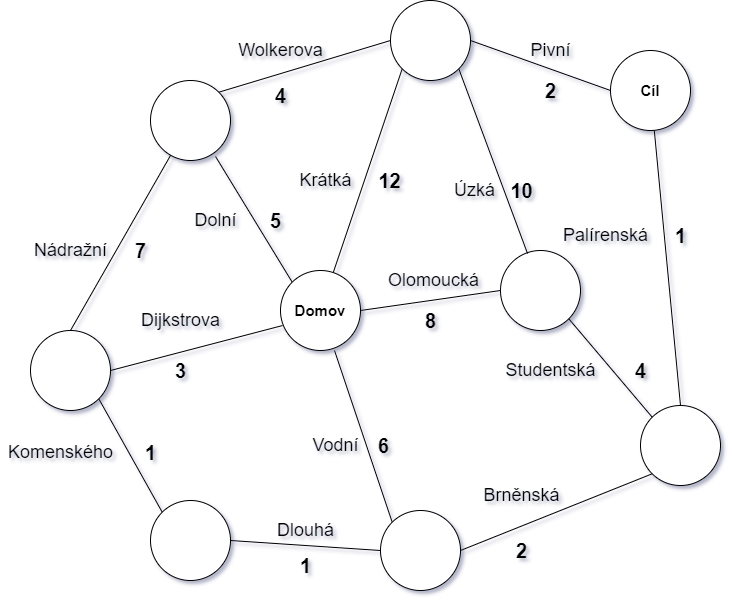
\includegraphics[scale=0.35]{Dijkstra.png}
}

\frame {
    \frametitle{Jaký problém řeší Dijkstrův algoritmus?}
    %\bigskip
    Jak v takovém grafu města najdeme nejkratší cestu z domova do našeho cíle -- třeba oblíbené hospůdky? \\[0.5em]
    Odpovědí je \textbf{Dijkstrův algoritmus}! \\ [0.5em]
    \begin{itemize}
        \item \textbf{Dijkstrův algoritmus} řeší problém nalezení nejkratší cesty grafem
        \item Základní princip:
        \begin{itemize}
            \setlength\itemsep{0.4em}
            \item Algoritmus ví, které vrcholy už navštívil a které ne, ke každému si pamatuje délku nejkratší cesty od výchozího vrcholu (na začátku jsou všechny $\infty$ daleko)
            \item Postupně ze seznamu nenavštívených vrcholů vybírá nejbližší z nich, zkoumá hrany, které z něj vedou a \uv{vylepšuje} vzdálenost bodů za těmito hranami
            \item \uv{Vylepšení} = pokud se mohu touto hranou dostat k bodu kratší cestou, pak dopočítám vzdálenost podle této hrany, pokud ne, hranu dále neřeším
            \item Tato činnost se opakuje, dokud neohodnotí celý graf nebo dokud nenavštívíme cílový vrchol
        \end{itemize}
    \end{itemize}
}

\frame {
\frametitle{Pseudokód algoritmu}
    \begin{adjustwidth}{0.5em}{-0.5em}
        \begin{algorithm}[H]
        \caption{\textsc{Dijkstrův algoritmus}}
            \DontPrintSemicolon
            \SetKwInput{KwInput}{Vstup}
            \SetKwInput{KwOutput}{Výstup}
            \KwInput{Vrcholy V, hrany E, počáteční a koncový vrchol S a F}
            \KwOutput{Ohodnocení vrcholů vzdálenostmi a cestou k vrcholu S}
            \BlankLine
            \For{$v \in V$}{
                v.distance = $\infty$\;
                v.previous = $None$ \; 
            }
            S.distance = 0\;
            unvisited = V \;
            \While{unvisited.count != 0}{
                best = getRemoveMinimal(unvisited) \; 
                \For{neighbor N $\in$ best.neighbors}{
                    newDist = best.distance + edgeLen(best,N) \; 
                    \If{newDist \textless\ N.distance}{
                        neighbor.distance = newDist \; 
                        neighbor.previous = best \; 
                        }
                    
                }
            }
        \end{algorithm}
    \end{adjustwidth}
}

\frame {
    \frametitle{Složitost algoritmu}
    \begin{itemize}
        \item Časová složitost Dijkstrova algoritmu záleží hlavně na datové struktuře použité pro uložení nenavštívených vrcholů
        \begin{itemize}
            \item Ve struktuře potřebujeme efektivně vyhledat a vybrat nejbližší vrchol
            \item Mezi možné struktury patří např. vázaný seznam, prioritní fronta, samovyvažující se binární stromy nebo seznam sousedů
        \end{itemize}
        \item Obecně je možné tuto složitost popsat jako funkci počtu hran a vrcholů, značí se $|E|$ resp. $|V|$
        \item Příklady složitosti při různých implementacích:
        \begin{itemize}
            \item Při nejjednodušší implementaci ve vázaném seznamu $\mathcal{O}(|V|^2)$
            \item Při implementaci v seznamu sousedů $\Theta(|V|^2 \log_2 |V|)$
            \item Při použití Fibonacciho haldy $\mathcal{O}(|E|+|V| \log_2 |V|)$
        \end{itemize}
    \end{itemize}
}

\frame {
    \frametitle{Příklad řešení cesty městem}
    \only<1>{
        \begin{block}{Příklad}
        Nejlépe algoritmus pochopíme obrázkem. Vyzkoušíme si jej na původním příkladu města. \\
        Změny ve vzdálenostech si vyznačíme \textbf{červeným číslem}, návštěvy \textbf{červenou šipkou}, vyřešené vrcholy \textbf{zeleně}. \\
        Pro zestručnění jsou uvedeny jen vybrané kroky algoritmu.
        \end{block}
    }
    \only<2>{
        \begin{exampleblock}{Krok 1}
        Začínáme ve výchozím bodě, najdeme vzdálenost všech sousedních bodů (křižovatek ve městě)
        \end{exampleblock}
        \begin{center}
            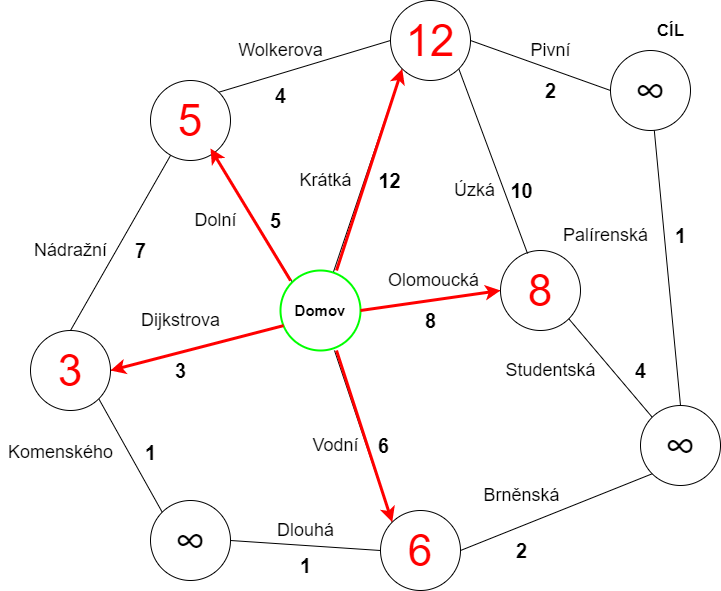
\includegraphics[scale=0.25]{img/Dijkstra1.png}
        \end{center}
    }
    \only<3>{
        \begin{exampleblock}{Krok 2}
        Nejblíže je křižovatka přes ulici \uv{Dijkstrova}, budeme zjišťovat vzdálenosti jejích sousedních bodů.
        \end{exampleblock}
        \begin{center}
            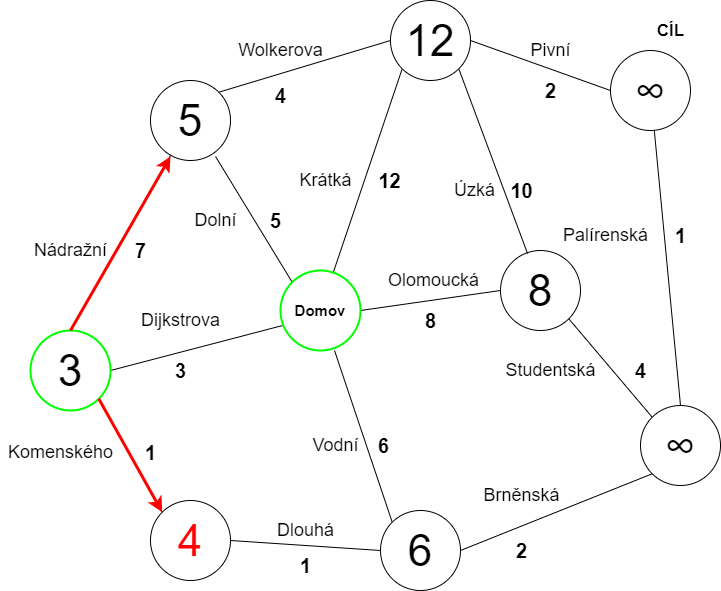
\includegraphics[scale=0.27]{img/Dijkstra2.png}
        \end{center}
    }
    \only<4>{
        \begin{exampleblock}{Krok 4}
        Postupně se dvěma kroky přes ulice \uv{Komenského} a \uv{Dlouhá} dostáváme k bodu, který už byl jednou ohodnocený, ale nalezli jsme k němu kratší cestu. Provedeme tedy \uv{vylepšení} a přiřadíme bodu nižší vzdálenost.
        \end{exampleblock}
        \begin{center}
            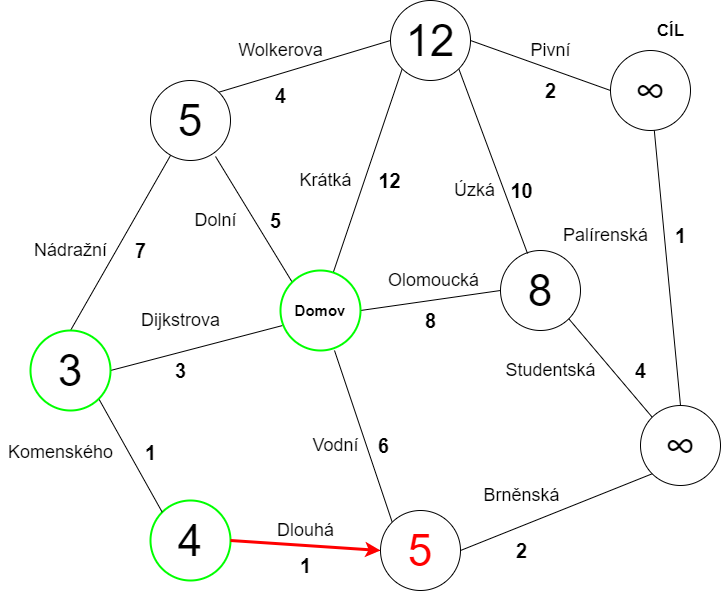
\includegraphics[scale=0.22]{img/Dijkstra3.png}   
        \end{center}
    }
    \only<5>{
        \begin{exampleblock}{Krok 6}
        O další dva kroky dále se dostáváme k našemu cíli.
        \end{exampleblock}
        \begin{center}
            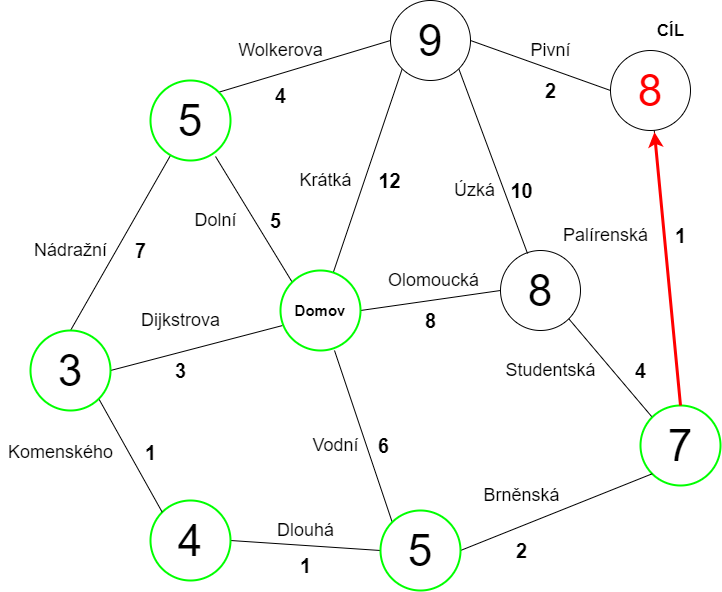
\includegraphics[scale=0.3]{img/Dijkstra4.png}    
        \end{center}
    }
    \only<6>{
        \begin{exampleblock}{Krok 9}
        Po ohodnocení cíle jsme ještě vybrali zbylé vrcholy, ale vzdálenosti již zůstaly stejné. \\
        Cestu jsme našli zpětně od cíle, protože jsme po cestě vázali vrcholy zpět k nejbližšímu.
        \end{exampleblock}
        \begin{center}
            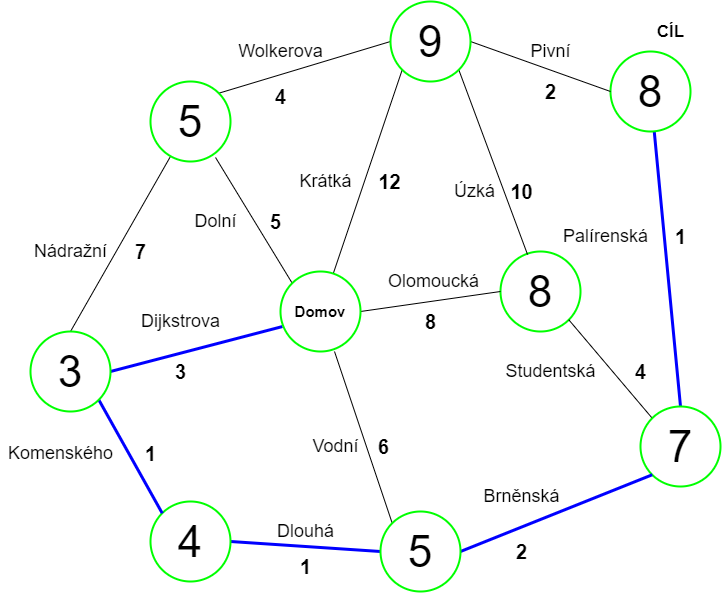
\includegraphics[scale=0.22]{img/Dijkstra5.png}    
        \end{center}
    }
}

\frame{
    \frametitle{Použité zdroje}
    \begin{itemize}
        \item Wikipedie: Dijkstrův algoritmus\\ \url{https://cs.wikipedia.org/wiki/Dijkstrův_algoritmus}
        \item Wikipedia: Dijkstra's algorithm\\ \url{https://en.wikipedia.org/wiki/Dijkstra\%27s_algorithm}
    \end{itemize}
}



\end{document}
